%!TEX root = ../2019_06_04-HATS-LPC-JEC.tex

\subsection{Introduction to Pileup}
%---------------------------------------------------------------------------------------------------------------------------------------
\begin{frame}[t]\frametitle{Outline}
    \begin{textblock}{0.65}(0.32,0.22)
    	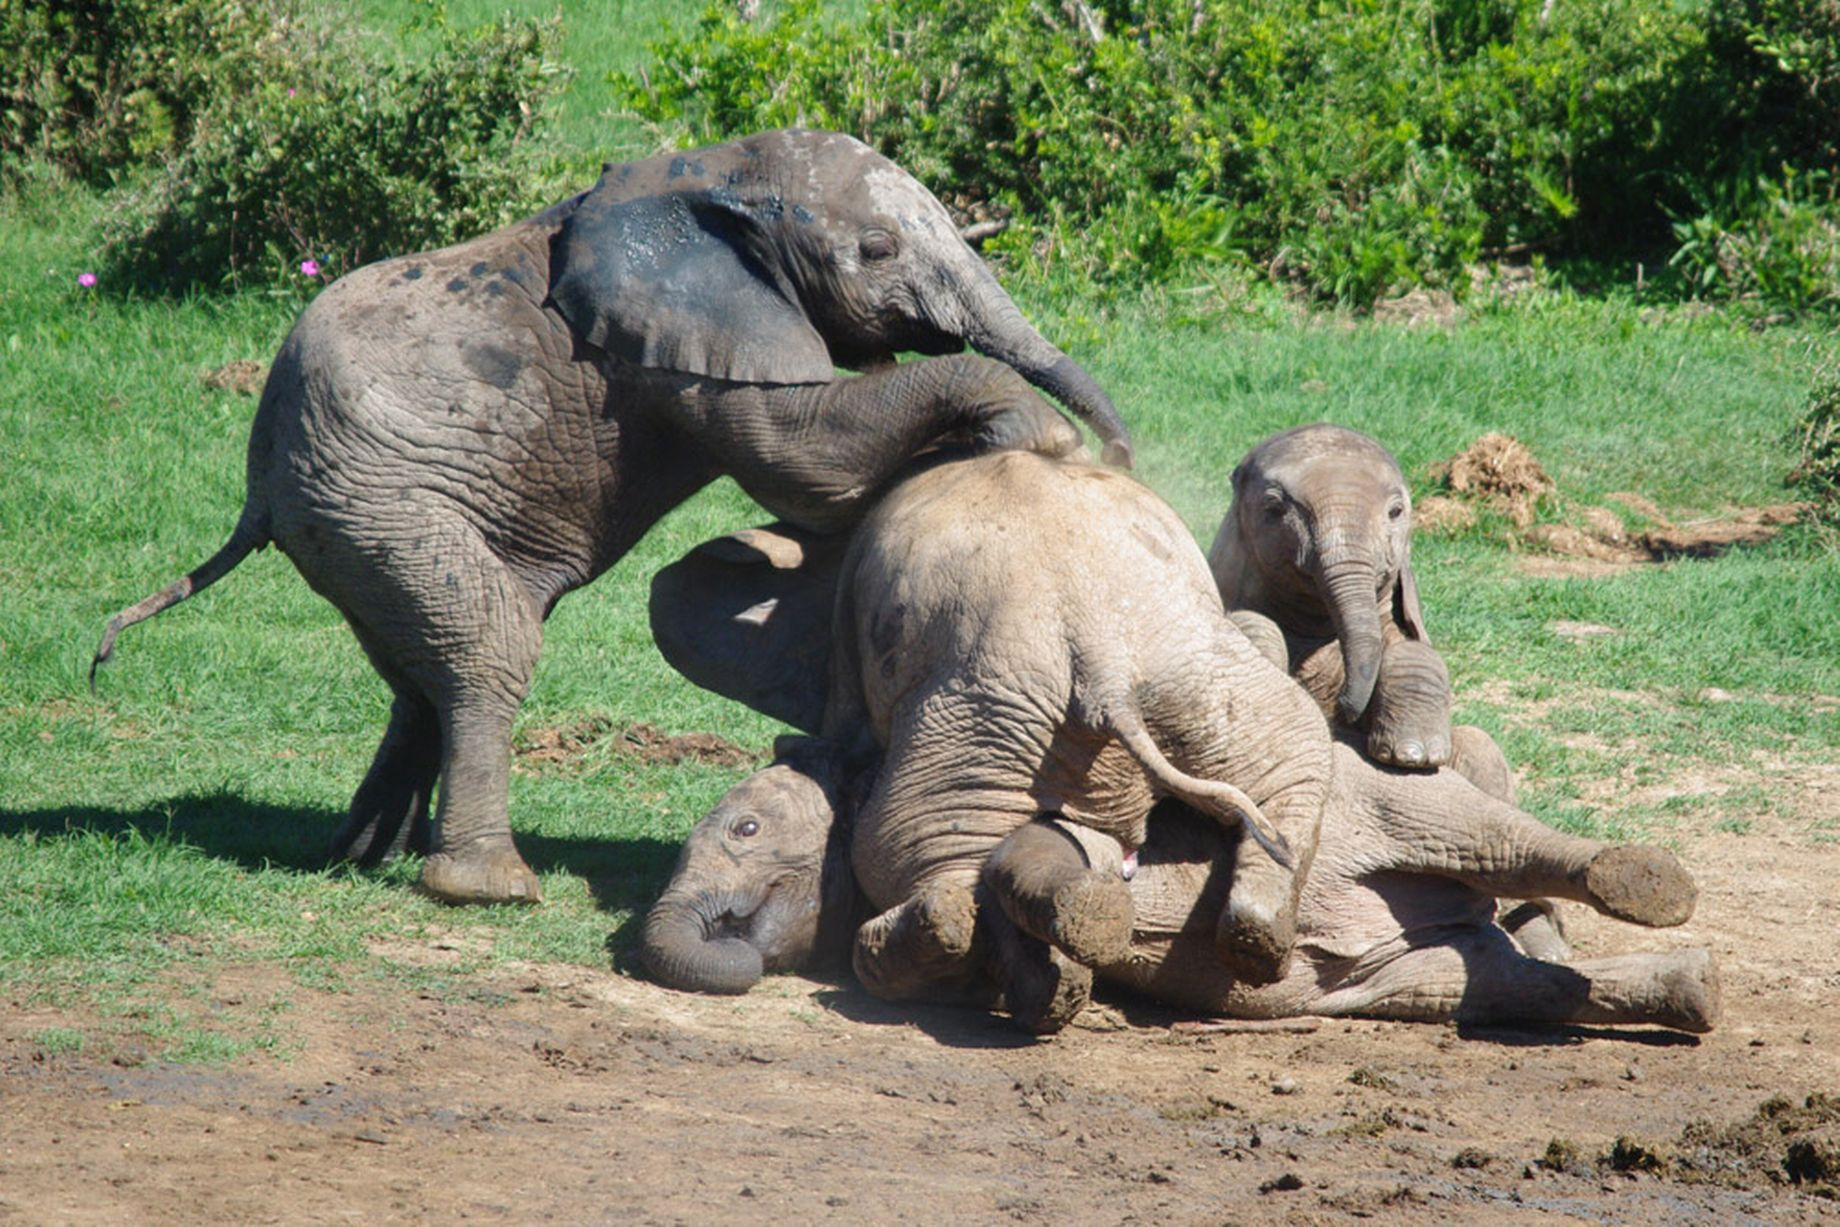
\includegraphics[width=\textwidth]{images/pileup/Elephant-Pile-Up.jpg}
    \end{textblock}

    \begin{textblock}{0.25}(0.04,0.3)
    	what is pileup?
    	\vspace*{1cm}

    	pileup reweighting
		\vspace*{1cm}

    	pileup mitigation\\~~focusing on PUPPI
    \end{textblock}
\end{frame}

\begin{frame}[t]\frametitle{Pileup: Definitions}
	\vspace*{-0.4cm}
	\begin{block}{Pileup}
		the \textbf{additional interactions} that occur in each beam crossing because the instantaneous bunch-by-bunch collision luminosity is very high
		\begin{itemize}
			\small
			\item ``additional'' implies that there is a hard-scatter interaction that has caused the event to fire the trigger
			\item the total inelastic cross section is approximately 80mb, so if the luminosity per collision is of order 80mb-1, you get one interaction per bunch crossing, on average
		\end{itemize}
	\end{block}
	\vspace*{-0.25cm}
	\begin{columns}[T]
		\begin{column}{0.48\textwidth}
			\vspace*{-0.15cm}
			\begin{exampleblock}{}
				\begin{customlist}{2.5em}{0em}
					\scriptsize
					\item \textbf{end of 2011:} ~15 interactions per crossing
					\item \textbf{2012:} as high as 40 interactions per crossing, mean of 21
					\item \textbf{2015:} as high as 40-50 interactions per crossing, mean of 13
					\item \textbf{2016:} as high as 60-70 interactions per crossing, mean of 27
					\item \textbf{2017:} as high as 80-90 interactions per crossing, mean of 38
					\item \textbf{2018:} as high as 100 interactions per crossing, mean of 37
				\end{customlist}
			\end{exampleblock}
		\end{column}
		\begin{column}{0.48\textwidth}
			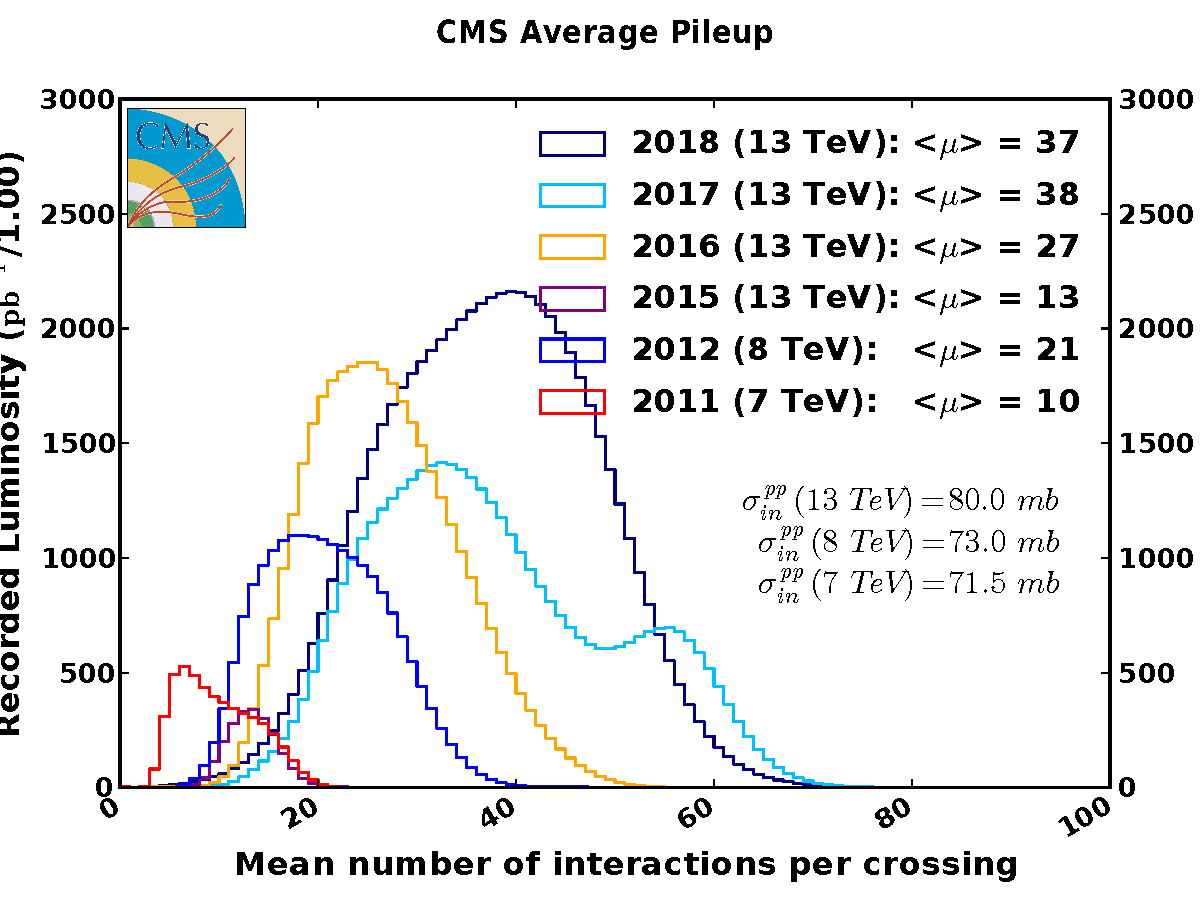
\includegraphics[width=\textwidth]{images/pileup/pileup_allYears.pdf}
		\end{column}
	\end{columns}
\end{frame}

\begin{frame}[t]\frametitle{Visualizing Pileup}
    \begin{textblock}{0.48}(0.01,0.3)
    	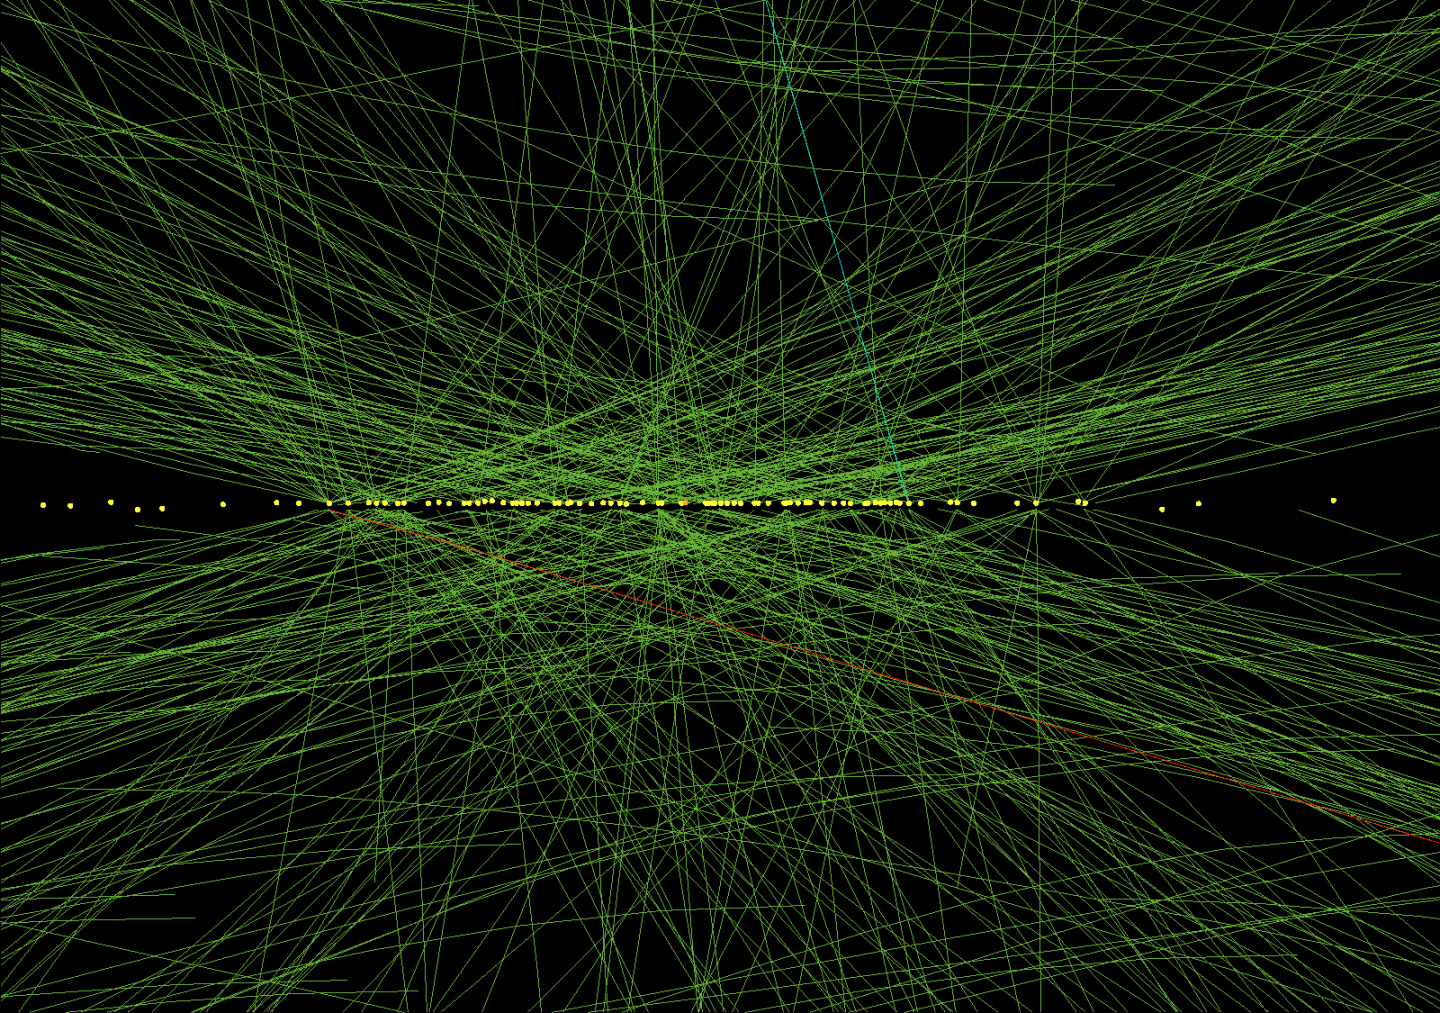
\includegraphics[width=\textwidth]{images/pileup/198609-56-3565522e.png}
    \end{textblock}
    \begin{textblock}{0.2}(0.28,0.56)
    	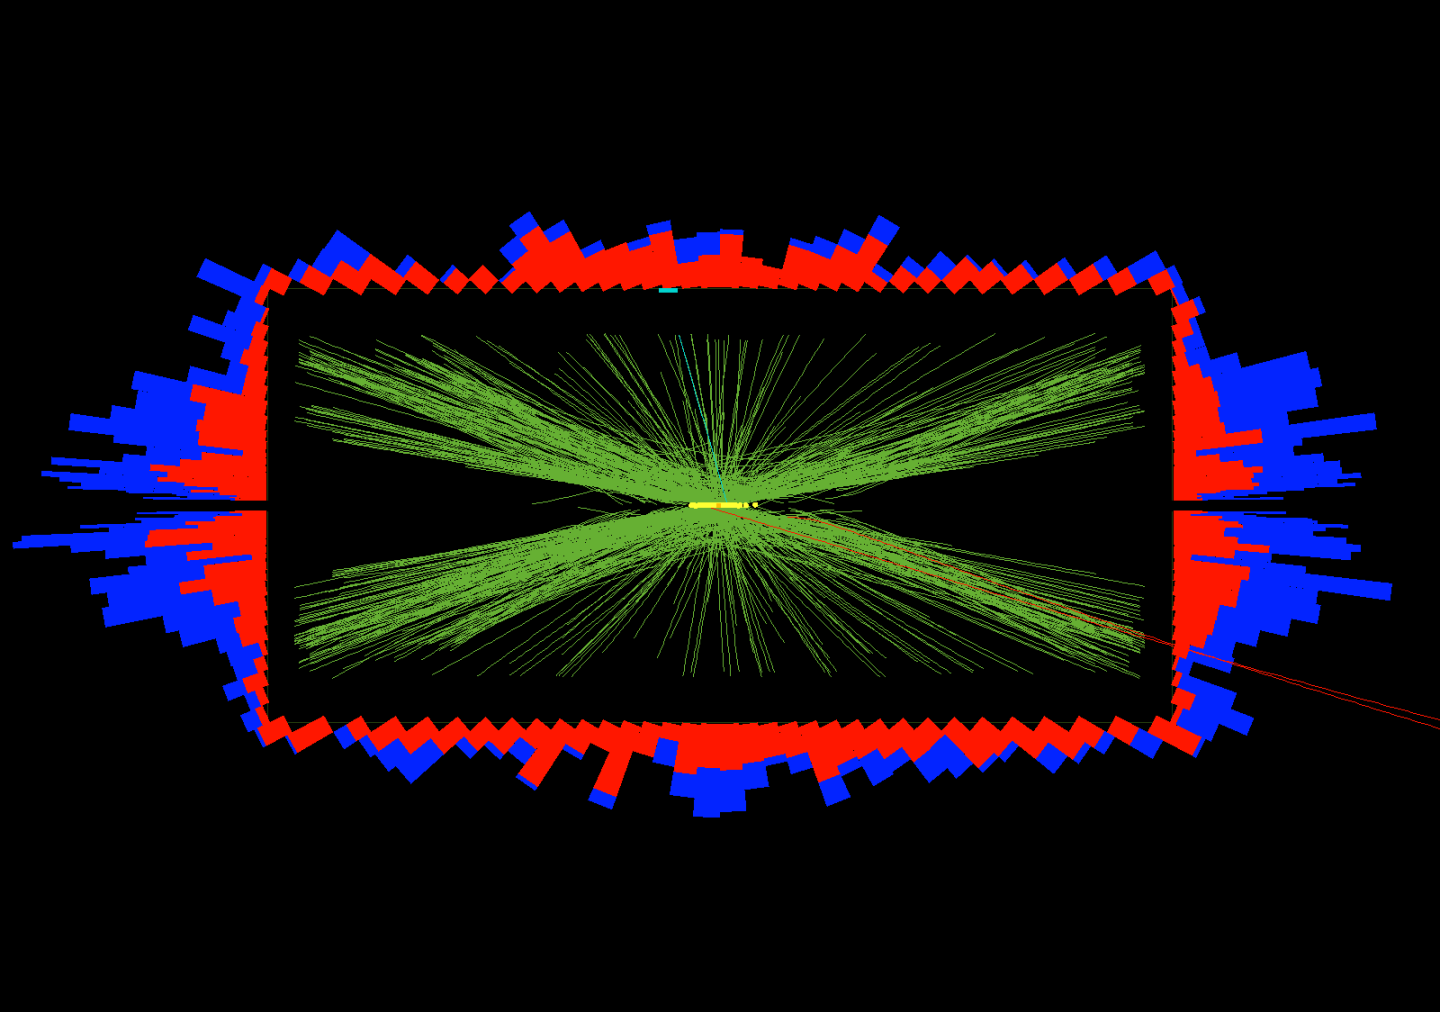
\includegraphics[width=\textwidth]{images/pileup/198609-56-3565522b.png}
    \end{textblock}
    \begin{textblock}{0.48}(0.5,0.13)
    	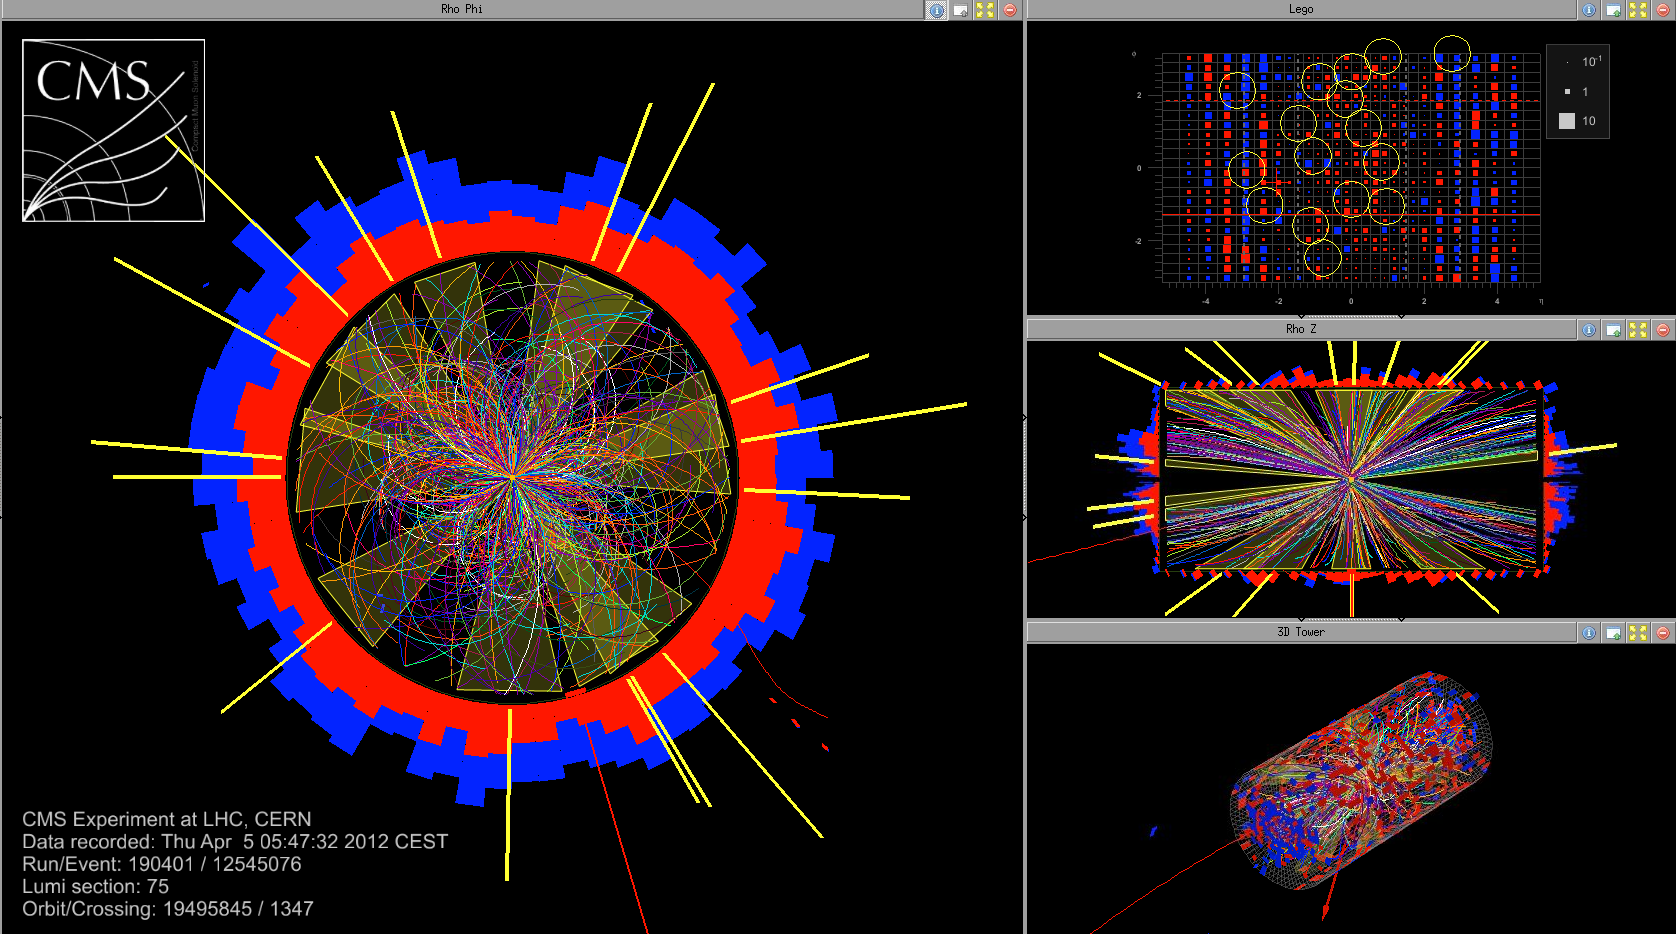
\includegraphics[width=\textwidth]{images/pileup/cms2012-2.png}
    	\vspace*{0.15cm}

    	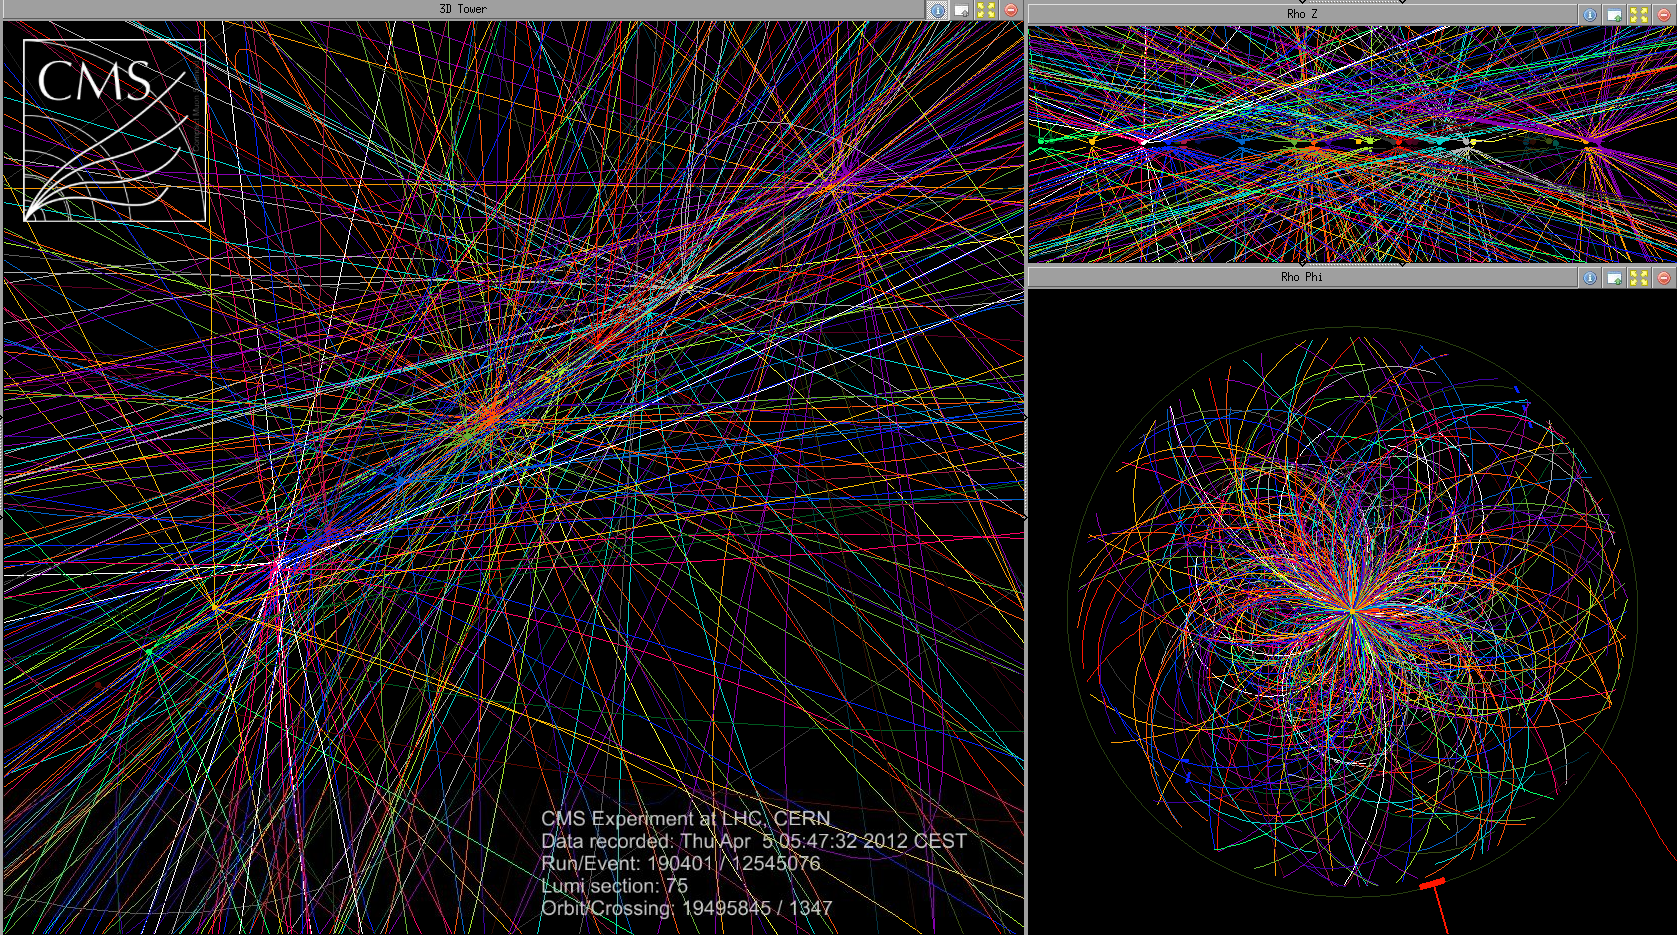
\includegraphics[width=\textwidth]{images/pileup/cms2012-3.png}
    \end{textblock}
\end{frame}

\begin{frame}[t]\frametitle{Pileup: Definitions}
	\vspace*{-0.45cm}
    \begin{block}{Types}
	    \textbf{In-time pileup:}
    	\begin{customlist}{2.5em}{0em}
    		\small
    	    \item the interactions that occur in the bunch crossing that fires the trigger
    	\end{customlist}
    	\textbf{Out-of-time pileup:}
    	\begin{customlist}{2.5em}{0em}
    		\small
    	    \item the interactions that occur in bunch crossings earlier or later than the in-time interaction
    	    \item depending on the integration time of the different CMS detector elements, these interactions can leave energy or tracks in the detector
    	\end{customlist}
    \end{block}
    \begin{textblock}{0.5}(0.02,0.52)
    	\begin{exampleblock}{Detector Elements}
    		\begin{customlist}{2.5em}{0em}
    			\scriptsize
    		    \item Tracker: only sensitive to in-time pileup
    		    \item Calorimeters: sensitive to out-of-time pileup
    		    \item Muons chambers: sensitive to out-of-time pileup
    		\end{customlist}
    	\end{exampleblock}
    	{\color{ForestGreen}Need to simulate out-of-time interactions, time structure of detector sensitivity and read-out, and bunch train structure}
    \end{textblock}
    \begin{textblock}{0.37}(0.59,0.54)
    	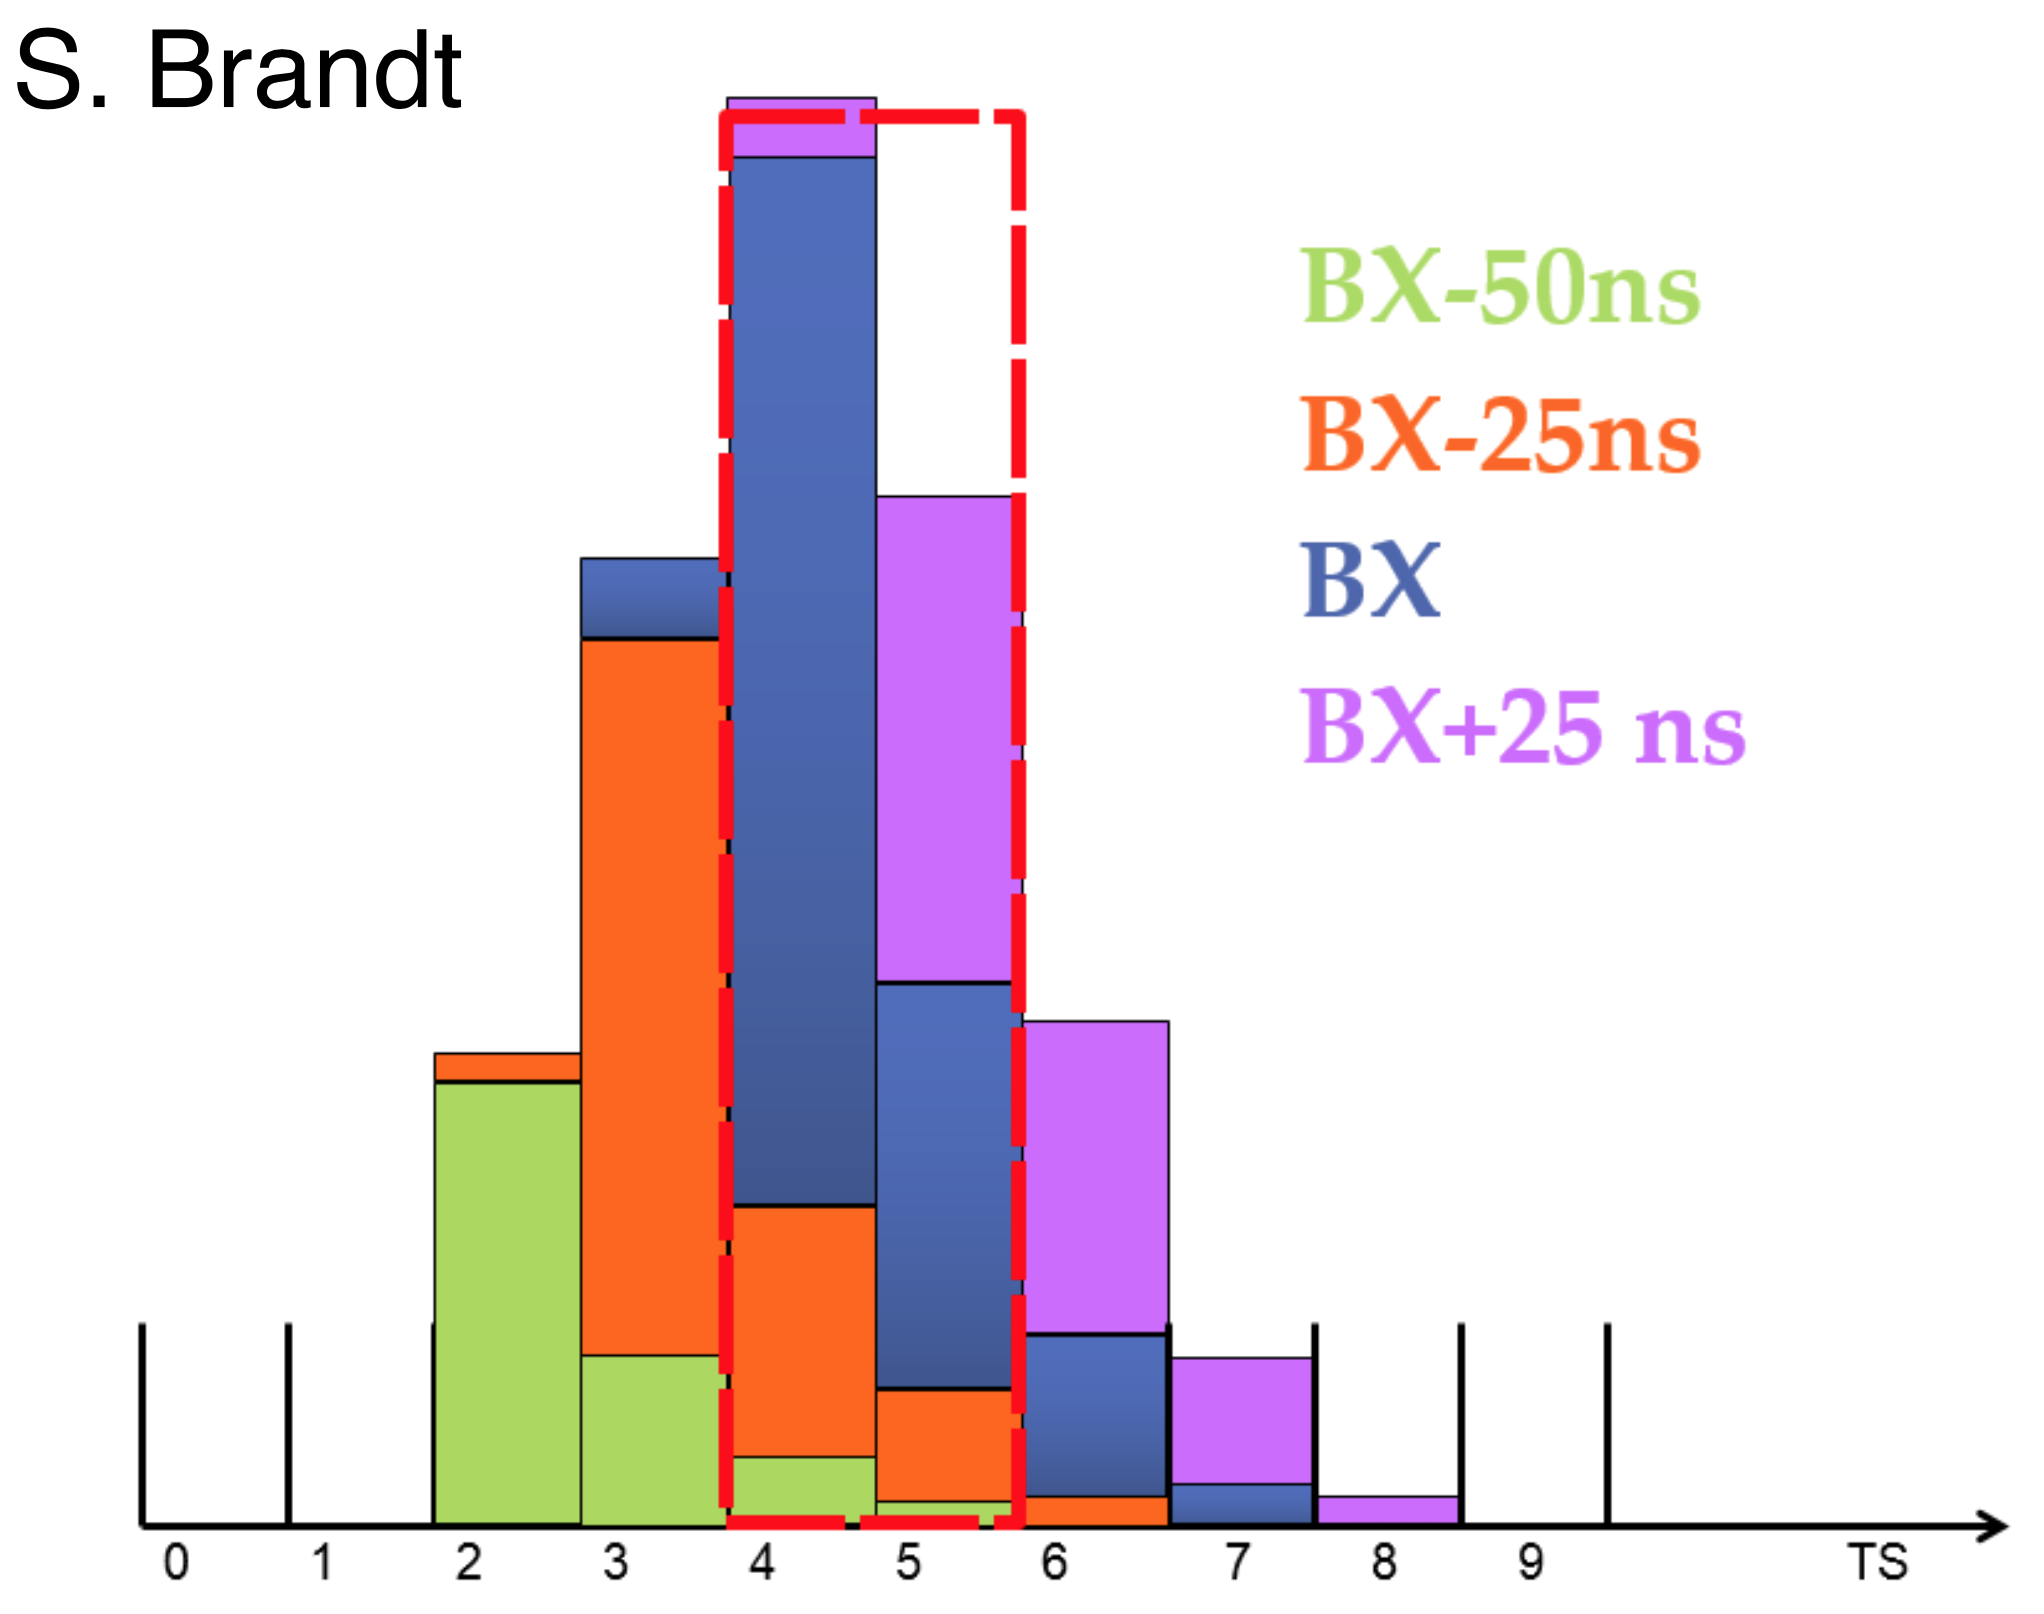
\includegraphics[width=\textwidth]{images/pileup/HCALPulse.png}
    \end{textblock}
\end{frame}